\documentclass{standalone}
\usepackage{tikz}
\usepackage{pgfplots}
\pgfplotsset{compat=1.11}
\definecolor{forestgreen}{rgb}{0.133, 0.545, 0.133}

\begin{document}
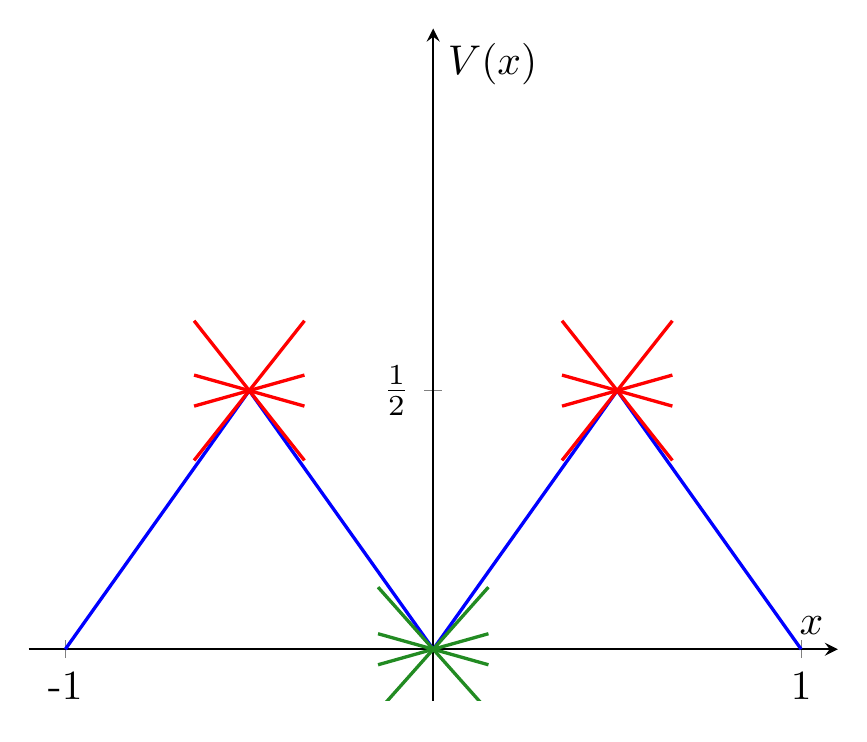
\begin{tikzpicture}[scale=1.5]
\begin{axis}[
xmin=-1.1,
xmax=1.1,
ymin=-0.1,
ymax=1.2,
grid=none,
axis lines=middle,
xlabel={$x$},          
ylabel={$V(x)$},   
yticklabels={0,$\frac12$},
ytick={0,.5},            
xticklabels={-1,0,1},
xtick={-1,0,1}, 
]
\addplot[blue,thick,domain=0:1]({x},{.5-abs(0.5-x)});
\addplot[blue,thick,domain=-1:0]({x},{.5-abs(0.5+x)});
\addplot[red,thick,domain=-0.65:-.35]({x},{0.5-0.2*(x+0.5)});
\addplot[red,thick,domain=-0.65:-.35]({x},{0.5+0.2*(x+0.5)});
\addplot[red,thick,domain=-0.65:-.35]({x},{0.5-0.9*(x+0.5)});
\addplot[red,thick,domain=-0.65:-.35]({x},{0.5+0.9*(x+0.5)});

\addplot[red,thick,domain=0.35:.65]({x},{0.5-0.2*(x-0.5)});
\addplot[red,thick,domain=0.35:.65]({x},{0.5+0.2*(x-0.5)});
\addplot[red,thick,domain=0.35:.65]({x},{0.5-0.9*(x-0.5)});
\addplot[red,thick,domain=0.35:.65]({x},{0.5+0.9*(x-0.5)});

\addplot[forestgreen,thick,domain=-0.15:0.15]({x},{.8*x});
\addplot[forestgreen,thick,domain=-0.15:0.15]({x},{-.8*x});
\addplot[forestgreen,thick,domain=-0.15:0.15]({x},{.2*x});
\addplot[forestgreen,thick,domain=-0.15:0.15]({x},{-.2*x});
\end{axis}
\end{tikzpicture}

\end{document}